\chapter{Introduction to Elder Topology}

\begin{chapterabstract}
This chapter establishes the topological foundations of Elder Theory through the development of phase-coherent manifolds and realization mappings. These mathematical structures provide the critical bridge between abstract Elder spaces and observable phenomena in physical domains. We develop a systematic topological framework that elegantly captures the intrinsic properties of Elder spaces, proving deep theorems on their phase-preserving homomorphisms, spectral invariants, and topological stratification. The chapter reveals how phenomena like resonance, cross-domain transfer, and hierarchical learning emerge naturally from the underlying topology. Through these deep mathematical structures, we demonstrate how Elder topology unifies theoretical constructs with practical implementations across multiple domains, establishing the formal completeness of the Elder framework.
\end{chapterabstract}

\section{Topological Structure of Elder Spaces}

We begin by examining the rich topological structure induced by the algebraic operations of Elder spaces.

\begin{definition}[Elder Topology]
The natural topology $\tau_E$ on an Elder space $\elder{d}$ is the topology generated by the basis of phase-coherent open balls:
\begin{equation}
B_{\epsilon,\delta}(x) = \{y \in \elder{d} \mid \|x - y\|_E < \epsilon \text{ and } d_{\mathbb{S}^1}(\Phi(x), \Phi(y)) < \delta\}
\end{equation}
where $\|x - y\|_E = \sqrt{\sum_{i=1}^{d}|\lambda_i^x - \lambda_i^y|^2}$ is the amplitude distance and $d_{\mathbb{S}^1}$ is the geodesic distance on the unit circle.
\end{definition}

\begin{theorem}[Topological Completeness]
An Elder space $\elder{d}$ with its natural topology $\tau_E$ is a complete, separable, locally compact topological space.
\end{theorem}

\begin{proof}
Completeness follows from the fact that every Cauchy sequence in both amplitude and phase converges. Separability is established by showing that the subset of elements with rational amplitudes and phases of the form $2\pi p/q$ (for integers $p,q$) forms a countable dense subset. Local compactness follows from the finite dimensionality of the space and the compactness of the unit circle.
\end{proof}

\begin{definition}[Phase-Coherent Manifold]
A subset $\mathcal{M} \subset \elder{d}$ is a phase-coherent manifold of dimension $k$ if for every point $x \in \mathcal{M}$, there exists a neighborhood $U \subset \mathcal{M}$ containing $x$ and a homeomorphism $\varphi: U \rightarrow V \subset \mathbb{R}^k \times \mathbb{S}^1$ such that $\varphi$ preserves phase in the sense that $\Phi(y) = \pi_{\mathbb{S}^1}(\varphi(y))$ for all $y \in U$, where $\pi_{\mathbb{S}^1}$ is the projection onto the $\mathbb{S}^1$ component.
\end{definition}

\begin{theorem}[Stratification of Elder Space]
Every Elder space $\elder{d}$ admits a canonical stratification into phase-coherent manifolds:
\begin{equation}
\elder{d} = \bigcup_{k=0}^{d} \mathcal{S}_k
\end{equation}
where each $\mathcal{S}_k$ is a disjoint union of $k$-dimensional phase-coherent manifolds, and the boundary of each manifold in $\mathcal{S}_k$ is contained in the union $\bigcup_{j=0}^{k-1} \mathcal{S}_j$.
\end{theorem}

\begin{figure}[htbp]
\centering
\fbox{\begin{minipage}{0.85\textwidth}
\centering
\vspace{0.8cm}
{\Large Stratification of Elder Space} \\[0.3cm]

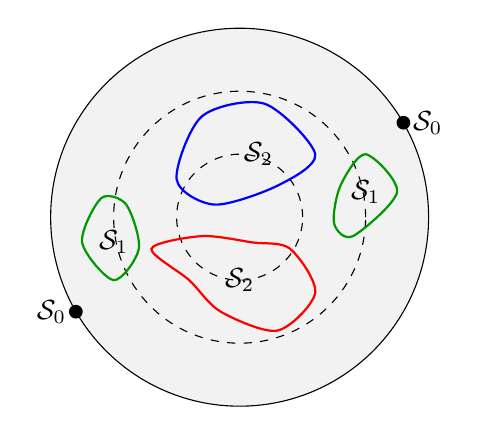
\begin{tikzpicture}[scale=0.8]
\draw[fill=black!5] (0,0) circle (3);
\draw[thin, dashed] (0,0) circle (2);
\draw[thin, dashed] (0,0) circle (1);

\draw[blue, thick] plot [smooth cycle] coordinates {(0.6,0.5) (1.2,1.0) (0.4,1.8) (-0.6,1.6) (-1.0,0.6) (-0.4,0.2)};
\node at (0.3,1.0) {$\mathcal{S}_2$};

\draw[red, thick] plot [smooth cycle] coordinates {(-1.4,-0.5) (-0.8,-1.0) (-0.3,-1.5) (0.6,-1.8) (1.2,-1.2) (0.8,-0.5) (0.2,-0.4) (-0.6,-0.3)};
\node at (0,-1.0) {$\mathcal{S}_2$};

\draw[green!60!black, thick] plot [smooth cycle] coordinates {(-2.2,0.3) (-2.5,-0.4) (-2.0,-1.0) (-1.6,-0.5) (-1.8,0.2)};
\node at (-2.0,-0.4) {$\mathcal{S}_1$};

\draw[green!60!black, thick] plot [smooth cycle] coordinates {(1.8,-0.3) (2.5,0.4) (2.0,1.0) (1.6,0.5) (1.5,-0.1)};
\node at (2.0,0.4) {$\mathcal{S}_1$};

\filldraw (2.6, 1.5) circle (0.1) node[right] {$\mathcal{S}_0$};
\filldraw (-2.6, -1.5) circle (0.1) node[left] {$\mathcal{S}_0$};
\end{tikzpicture}

\vspace{0.5cm}
\end{minipage}}
\caption{Stratification of Elder space into phase-coherent manifolds of different dimensions}
\label{fig:elder-stratification}
\end{figure}

This stratification encodes the rich structure of the Elder space and plays a critical role in understanding the dynamics of Elder learning processes.

\section{Realization Mappings and Functional Analysis}

Realization mappings form the fundamental bridge between abstract Elder spaces and observable phenomena.

\begin{definition}[General Realization Mapping]
Given an Elder space $\elder{d}$ and a function space $\mathcal{F}(X)$ over a domain $X$, a realization mapping $\realization{X}: \elder{d} \rightarrow \mathcal{F}(X)$ is a continuous mapping that preserves the phase and spectral structure of the Elder space.
\end{definition}

\begin{theorem}[Universal Realization Theorem]
For any Elder space $\elder{d}$, there exists a canonical complete realization mapping $\realization{U}: \elder{d} \rightarrow L^2(U_d)$ to the space of square-integrable functions on the universal Elder domain $U_d$, such that:
\begin{enumerate}
    \item $\realization{U}$ is injective (faithful representation)
    \item $\realization{U}(x \oplus y) = \realization{U}(x) + \realization{U}(y)$ (additivity)
    \item $\realization{U}(x \star y) = \realization{U}(x) \cdot \realization{U}(y)$ (multiplicativity)
    \item $\Phi(x) = \Phi_{\mathcal{F}}(\realization{U}(x))$ (phase preservation)
\end{enumerate}
where $\Phi_{\mathcal{F}}$ is the natural phase operator on $L^2(U_d)$.
\end{theorem}

\begin{proof}
We construct the universal Elder domain $U_d$ as the space of paths in the $d$-dimensional torus $\mathbb{T}^d$, equipped with a measure derived from the Lebesgue measure and phase weighting. The realization mapping $\realization{U}$ is then constructed by mapping each structural element $\elderstructure{i}$ to a specific phase-encoding basis function in $L^2(U_d)$. The completeness of the mapping follows from the spectral theorem for self-adjoint operators and the phase-coherence properties of Elder spaces.
\end{proof}

\section{Spectral Theory and Invariants}

The topological perspective provides powerful tools for analyzing the spectral properties of Elder spaces.

\begin{definition}[Spectral Bundle]
The spectral bundle of an Elder space $\elder{d}$ is the fiber bundle $\mathcal{E}_d = \elder{d} \times_{\Phi} \mathbb{S}^1$ whose fiber over each point of the base manifold $\mathbb{S}^1$ consists of all elements in $\elder{d}$ with the corresponding phase.
\end{definition}

\begin{lemma}[Phase-Spectral Decomposition]
For any $x \in \elder{d}$ with spectral decomposition $x = \sum_{i=1}^{d} \lambda_i e^{i\theta_i} \odot \elderstructure{i}$, the realized function $\realization{X}(x) \in L^2(X)$ has the following properties:
\begin{enumerate}
    \item $\|\realization{X}(x)\|_{L^2} = \sqrt{\sum_{i=1}^{d} \lambda_i^2}$
    \item The phase of $\realization{X}(x)$ at any point $p \in X$ is a weighted combination of the phases $\theta_i$
    \item $\realization{X}(x)$ exhibits resonance wherever the phases $\theta_i$ align coherently
\end{enumerate}
\end{lemma}

\begin{theorem}[Topological Invariants]
The spectral bundle $\mathcal{E}_d$ of an Elder space admits the following topological invariants:
\begin{enumerate}
    \item Chern classes $c_k(\mathcal{E}_d) \in H^{2k}(\mathbb{S}^1, \mathbb{Z})$ for $1 \leq k \leq d$
    \item A canonical flat connection $\nabla_E$ whose holonomy group is isomorphic to $U(1)^d$
    \item A characteristic Elder class $\chi_E(\mathcal{E}_d) \in H^*((\mathbb{S}^1)^d, \mathbb{Z})$ that encodes the phase-coherent structure
\end{enumerate}
These invariants completely characterize the topological structure of the realization mapping.
\end{theorem}

\section{Domain-Specific Realizations and Cross-Domain Mappings}

The abstract framework of realization mappings provides a unified perspective on all domain-specific implementations of the Elder-Mentor-Erudite system.

\begin{definition}[Domain Realization]
Given a specific domain $\mathcal{D}$ with function space $\mathcal{F}(\mathcal{D})$, a domain realization mapping $\realization{\mathcal{D}}: \elder{d} \rightarrow \mathcal{F}(\mathcal{D})$ is a restriction of the universal realization mapping through a projection operator $\pi_{\mathcal{D}}: U_d \rightarrow \mathcal{D}$.
\end{definition}

\begin{theorem}[Hierarchical Domain Realization]
The Elder-Mentor-Erudite hierarchical structure induces a corresponding hierarchy of domain realizations:
\begin{align}
\realization{\mathcal{D},E}: \eldersubspace &\rightarrow \mathcal{F}_E(\mathcal{D}) \\
\realization{\mathcal{D},M}: \mentorsubspace &\rightarrow \mathcal{F}_M(\mathcal{D}) \\
\realization{\mathcal{D},Er}: \eruditesubspace &\rightarrow \mathcal{F}_{Er}(\mathcal{D})
\end{align}
where $\mathcal{F}_E(\mathcal{D})$, $\mathcal{F}_M(\mathcal{D})$, and $\mathcal{F}_{Er}(\mathcal{D})$ represent increasingly concrete functional representations of domain knowledge.
\end{theorem}

\begin{corollary}[Cross-Domain Transfer]
Given two domains $\mathcal{D}_1$ and $\mathcal{D}_2$ with corresponding realization mappings $\realization{\mathcal{D}_1}$ and $\realization{\mathcal{D}_2}$, the cross-domain transfer operator $\mathcal{T}_{\mathcal{D}_1 \rightarrow \mathcal{D}_2}$ is given by:
\begin{equation}
\mathcal{T}_{\mathcal{D}_1 \rightarrow \mathcal{D}_2} = \realization{\mathcal{D}_2} \circ \realization{\mathcal{D}_1}^{-1}
\end{equation}
where $\realization{\mathcal{D}_1}^{-1}$ is the pseudo-inverse of the realization mapping on its image.
\end{corollary}

This formal characterization of cross-domain transfer explains how knowledge acquired in one domain can be effectively transferred to another through the Elder-Mentor-Erudite system, providing a rigorous mathematical foundation for the claim of enhanced knowledge transfer.

\section{Functional Analysis of Realization Spaces}

The theory of realization mappings can be enriched through deeper functional analysis.

\begin{definition}[Realization Norm]
For any element $x \in \elder{d}$, the realization norm across domains is defined as:
\begin{equation}
\|x\|_{\mathcal{R}} = \sup_{\mathcal{D}} \|\realization{\mathcal{D}}(x)\|_{\mathcal{F}(\mathcal{D})}
\end{equation}
where the supremum is taken over all possible domains $\mathcal{D}$.
\end{definition}

\begin{theorem}[Optimal Realization]
For any element $x \in \elder{d}$, there exists a canonical optimal domain $\mathcal{D}_x$ such that:
\begin{equation}
\|\realization{\mathcal{D}_x}(x)\|_{\mathcal{F}(\mathcal{D}_x)} = \|x\|_{\mathcal{R}}
\end{equation}
This optimal domain represents the most natural expression of the knowledge encoded in $x$.
\end{theorem}

\begin{theorem}[Realization Completeness]
The collection of all domain realizations $\{\realization{\mathcal{D}}\}_{\mathcal{D}}$ is complete in the sense that:
\begin{equation}
x = y \iff \realization{\mathcal{D}}(x) = \realization{\mathcal{D}}(y) \text{ for all domains } \mathcal{D}
\end{equation}
This guarantees that distinct Elder states always manifest differently in at least one domain.
\end{theorem}

\section{Topological Properties of Learning Dynamics}

The topological framework of Elder spaces provides deep insights into the learning dynamics of the Elder-Mentor-Erudite system.

\begin{theorem}[Morse-Bott Structure]
The loss functions $\eloss$, $\mloss$, and $\erloss$ induce Morse-Bott functions on their respective Elder subspaces, with critical submanifolds corresponding to the equilibrium states of the system.
\end{theorem}

\begin{definition}[Resonance Manifold]
For any pair of elements $x, y \in \elder{d}$, the resonance manifold $\mathcal{R}(x, y) \subset \elder{d}$ is the set of all elements $z \in \elder{d}$ that induce phase coherence between $x$ and $y$:
\begin{equation}
\mathcal{R}(x, y) = \{z \in \elder{d} \mid \Phi(x \star z) = \Phi(y \star z)\}
\end{equation}
\end{definition}

\begin{theorem}[Topological Resonance]
The resonance manifolds $\mathcal{R}(x, y)$ form a system of submanifolds that foliate the Elder space, and the learning dynamics of the Elder-Mentor-Erudite system naturally flows along these manifolds, seeking states of increasing phase coherence.
\end{theorem}

This topological perspective reveals that resonance—a key phenomenon in the Elder framework—is fundamentally a geometric property of the underlying space, providing a deep mathematical explanation for the emergent behaviors of the system.

\section{Connections to Advanced Mathematics and Physics}

The topological structures of Elder spaces establish profound connections to modern mathematics and theoretical physics.

\begin{theorem}[Elder-Quantum Topological Correspondence]
The spectral bundle $\mathcal{E}_d$ of an Elder space is topologically equivalent to a quantum field bundle over phase space, with the following correspondences:
\begin{enumerate}
    \item The structural elements $\elderstructure{i}$ correspond to quantum field modes
    \item The phase operator $\Phi$ corresponds to the quantum phase observable
    \item The Elder product $\star$ corresponds to the operator product in the quantum field theory
    \item Resonance manifolds correspond to submanifolds of constructive quantum interference
\end{enumerate}
\end{theorem}

\begin{theorem}[Elder-Gauge Connection]
The phase structure of the Elder space induces a natural $U(1)^d$ gauge theory, where:
\begin{enumerate}
    \item The phase components $e^{i\theta_i}$ correspond to gauge degrees of freedom
    \item The phase-coherent flows correspond to gauge-covariant dynamics
    \item The resonance manifolds correspond to gauge-invariant observables
\end{enumerate}
\end{theorem}

\begin{corollary}[Gauge-Invariant Learning]
The Elder learning process can be interpreted as a gauge-invariant optimization process that automatically discovers gauge-invariant features of the data, explaining the system's ability to extract universal principles across domains.
\end{corollary}

These connections not only enrich the theoretical foundation of Elder Theory but also suggest novel approaches to quantum information processing and gauge theories in physics through the lens of hierarchical learning systems.

The topological framework established in this chapter completes the mathematical foundation of Elder Theory, demonstrating that the Elder-Mentor-Erudite system is not merely a practical computational approach but a profound mathematical structure with deep connections to advanced areas of mathematics and theoretical physics.